\section{Code-Beispiele}
\label{sec:12-code-beispiele}

\subsection{Sortieralgorithmen}
\label{sec:12-sortieralgorithmen}


\subsubsection{Quick Sort (Median-of-Three Pivot)}
\begin{codebox}
\begin{lstlisting}[style=CodeExpert]
def quicksort_median3_pivot(A, left, right):
    if left < right:
        mid = (left + right) // 2
        if A[mid] < A[left]:
            A[left], A[mid] = A[mid], A[left]
        if A[right] < A[left]:
            A[left], A[right] = A[right], A[left]
        if A[right] < A[mid]:
            A[mid], A[right] = A[right], A[mid]

        pivot = A[mid]
        i = left
        j = right - 1
        while i < j:
            while i <= j and A[i] <= pivot:
                i += 1
            while i <= j and A[j] >= pivot:
                j -= 1
            if i < j:
                A[i], A[j] = A[j], A[i]
        A[left], A[j] = A[j], A[left]
        quicksort_median3_pivot(A, left, j)
        quicksort_median3_pivot(A, j + 1, right)
\end{lstlisting}
\end{codebox}

\subsubsection{Merge Sort}
\begin{codebox}
\begin{lstlisting}[style=CodeExpert]
def merge_sort(a):
    if len(a) == 1:
        return a
    else:
        s1 = merge_sort(a[:len(a)//2])
        s2 = merge_sort(a[len(a)//2:])
        s = merge(s1, s2)
        return s
def merge(a1, a2):
    b, i, j = [], 0, 0
    while i < len(a1) and j < len(a2):
        if a1[i] < a2[j]:
            b.append(a1[i])
            i += 1
        else:
            b.append(a2[j])
            j += 1
    b += a1[i:]
    b += a2[j:]
    return b
\end{lstlisting}
\end{codebox}


\subsubsection{Insertion Sort}
\begin{codebox}
\begin{lstlisting}[style=CodeExpert]
def insertionSort(A, l, r):
    for i in range(l + 1, r):
        j = i - 1
        while j >= 0 and A[j] > A[j + 1]:
            A[j], A[j + 1] = A[j + 1], A[j]
            j -= 1
\end{lstlisting}
\end{codebox}

\subsubsection{Bubble Sort}
\begin{codebox}
\begin{lstlisting}[style=CodeExpert]
def bubbleSort(A, l, r):
    for i in range(l, r):
        for j in range(r - i - 1):
            if A[j] > A[j + 1]:
                swap(A, j, j + 1)
\end{lstlisting}
\end{codebox}


\subsubsection{Selection Sort}
\begin{codebox}
\begin{lstlisting}[style=CodeExpert]
def selectionSort(A, l, r):
    for i in range(l, r):
        minJ = i
        for j in range(i + 1, r):
            if A[j] < A[minJ]:
                minJ = j
        if minJ != i:
            A[i], A[minJ] = A[minJ], A[i]
\end{lstlisting}
\end{codebox}


\subsubsection{Binary Insertion Sort}
\begin{codebox}
\begin{lstlisting}[style=CodeExpert]
# This function will return the index of element
# just greater than 'key' in Array from 0-N
def binarySearch(Array, N, key):
    L = 0
    R = N
    while (L < R):
        mid = (L + R) // 2
        if (Array[mid] <= key):
            L = mid + 1
        else:
            R = mid
    return L

def binaryInsertionSort(Array):
    # We assume the 1st element of Array to be already sorted.
    # Start iterating from the 2nd element to the last element.
    for i in range(1, len(Array)):
        key = Array[i]
        pos = binarySearch(Array, i, key)
        # 'pos' will now contain the index
        # where 'key' should be inserted.
        j = i
        # Shifting every element from 'pos' to 'i' towards right
        while (j > pos):
            Array[j] = Array[j - 1]
            j -= 1
        # Inserting 'key' in its correct position.
        Array[pos] = key
        print("The array after", i, "iterations =>", *Array)
\end{lstlisting}
\end{codebox}

\subsubsection{Heap Sort}
\begin{codebox}
\begin{lstlisting}[style=CodeExpert]
def heap_sort(list):
    # turns list into valid heap
    heapify(list)

    for i in reversed(range(len(list))):
        list[0], list[i] = list[i], list[0]
        siftDown(list, 0, i)

    return
\end{lstlisting}
\end{codebox}



\subsection{Dynamische Programmierung und Memo}
\label{sec:12-dp-memoization}



%=====================================================================================================================
\subsubsection{Karotten in $n\times n$ Matrix: Bester Weg}
\begin{codebox}
\begin{lstlisting}[style=CodeExpert]
def longest_path_dp(grid):
    n, m = len(grid), len(grid[0])
    s = [[None] * m for _ in range(n)]
    decision = [[None] * m for _ in range(n)]

    # fill out the DP table:
    for i in range(n - 1, -1, -1):
        for j in range(m - 1, -1, -1):
            if i == n - 1 and j == m - 1:
                s[i][j] = grid[i][j]
                decision[i][j] = "Stop"
            elif i == n - 1 and j < m - 1:
                s[i][j] = grid[i][j] + s[i][j + 1]
                decision[i][j] = "East"
            elif i < n - 1 and j == m - 1:
                s[i][j] = grid[i][j] + s[i + 1][j]
                decision[i][j] = "South"
            else:
                east = grid[i][j] + s[i][j + 1]
                south = grid[i][j] + s[i + 1][j]
                s[i][j] = max(east, south)
                decision[i][j] = "East" if east >= south
                else "South"

    # reconstruct the best path:
    path, i, j = [], 0, 0
    while (i, j) != (n - 1, m - 1):
        path.append(decision[i][j])
        if decision[i][j] == "East":
            j += 1
        else:
            i += 1

    return s[0][0], path
\end{lstlisting}
\end{codebox}

\subsubsection{Treppensteigen (DP) — Anzahl Wege}
\begin{codebox}
\begin{lstlisting}[style=CodeExpert]
# How many distict ways are there to climb
# n number of stairs if you tiake on or two steps at a time
def climb_stairs(n: int) -> int:
    a, b = 1, 1
    for _ in range(n - 1):
        a, b = b, a + b
    return b

\end{lstlisting}
\end{codebox}

\subsubsection{Golomb-Zahlen (nur Rekursion)}
\begin{codebox}
\begin{lstlisting}[style=CodeExpert]
def golomb(n):
    """
    pre: integer n > 0
    post: return the nth Golomb number
    """
    if n == 1:
        return 1
    else:
        return 1 + golomb(n=golomb(golomb(n - 1)))
\end{lstlisting}
\end{codebox}




\subsubsection{Stab schneiden (Rod Cutting)}
\begin{codebox}
\begin{lstlisting}[style=CodeExpert]
# w: Liste mit Werten für Stabstückchenlänge
def cuts(n, w):
    s = [None] * (n + 1)
    L = [None] * (n + 1)

    for i in range(n + 1):
        if i == 0:
            s[i] = 0
        else:
            option = 1
            value = w[1] + s[i - 1]
            for j in range(1, i + 1):
                new_option = j
                new_value = w[j] + s[i - j]
                if new_value > value:
                    option = j
                    value = new_value
            s[i] = value
            L[i] = option

    i = n
    cut = []
    while i >= 1:
        cut.append(L[i])
        i -= L[i]

    return (s[n], cut)
\end{lstlisting}
\end{codebox}

\subsection{ML / Cross-Validation mit \texttt{GridSearchCV}}
\label{sec:12-ml-cross-validation}

\subsubsection{Imports}
\begin{codebox}
\begin{lstlisting}[style=CodeExpert]
import numpy as np
import pandas as pd
import matplotlib.pyplot as plt
import warnings
from sklearn.datasets import make_circles
from sklearn.model_selection import train_test_split, GridSearchCV
from sklearn.neural_network import MLPClassifier
from sklearn.linear_model import LogisticRegression
from sklearn.tree import DecisionTreeClassifier, plot_tree
from sklearn.metrics import accuracy_score
from utils import plot_decision_boundary, plot_data

\end{lstlisting}
\end{codebox}

\subsubsection{GridSearchCV — Anwendung}
\begin{codebox}
\begin{lstlisting}[style=CodeExpert]
# read in the data
df = pd.read_csv("data.csv")
X = df[["size", "bright"]].to_numpy()
y = df["label"].to_numpy()

# split the data into training and testing
X_train, X_test, y_train, y_test = train_test_split(
    X, y, test_size=0.5, random_state=42)

# Crossvalidate the different tree lengths using the train data
dt = DecisionTreeClassifier()
# tree depth from 1 to 9
grid = {"max_depth": range(1, 10)}

grid = GridSearchCV(dt, param_grid=grid, cv=5)
grid.fit(X_train, y_train)

best_dt = grid.best_estimator_

y_pred_train = best_dt.predict(X_train)
y_pred_test = best_dt.predict(X_test)

acc_train = accuracy_score(y_train, y_pred_train)
acc_test = accuracy_score(y_test, y_pred_test)

print("Accuracy on train data: {:.2f}".format(acc_train))
print("Accuracy on test data: {:.2f}".format(acc_test))
\end{lstlisting}
\end{codebox}




\subsubsection{Knapsack DP}
\begin{codebox}
\begin{lstlisting}[style=CodeExpert]
def knapsack(weights, values, capacity):
    n = len(weights)
    dp = [[0] * (capacity + 1) for _ in range(n + 1)]

    for i in range(1, n + 1):
        for w in range(capacity + 1):
            if weights[i-1] <= w:
                dp[i][w] = max(
                    dp[i-1][w],
                    dp[i-1][w - weights[i-1]] + values[i-1]
                )
            else:
                dp[i][w] = dp[i-1][w]

    return dp[n][capacity]
\end{lstlisting}
\end{codebox}




\subsubsection{Optimal Binary Search Tree DP}
\begin{codebox}
\begin{lstlisting}[style=CodeExpert]
def optimal_bst(freq):
    n = len(freq)
    dp = [[0]*n for _ in range(n)]
    sum_freq = [[0]*n for _ in range(n)]

    for i in range(n):
        sum_freq[i][i] = freq[i]
        for j in range(i+1, n):
            sum_freq[i][j] = sum_freq[i][j-1] + freq[j]

    for length in range(1, n+1):
        for i in range(n - length + 1):
            j = i + length - 1
            dp[i][j] = float('inf')
            for r in range(i, j+1):
                cost = (dp[i][r-1] if r > i else 0) + \
                       (dp[r+1][j] if r < j else 0) + \
                       sum_freq[i][j]
                dp[i][j] = min(dp[i][j], cost)

    return dp[0][n-1]
\end{lstlisting}
\end{codebox}


\subsubsection{Graph DP (Memoization)}
\begin{codebox}
\begin{lstlisting}[style=CodeExpert]
def graph_dp(node, graph, dp):
    if node in dp:
        return dp[node]

    if not graph[node]:  # leaf
        dp[node] = 0
        return 0

    max_cost = 0
    for neighbor, weight in graph[node]:
        cost = weight + graph_dp(neighbor, graph, dp)
        max_cost = max(max_cost, cost)

    dp[node] = max_cost
    return max_cost
\end{lstlisting}
\end{codebox}



\subsubsection{Longest Common Subsequence (LCS) — memoisiert}
\begin{codebox}
\begin{lstlisting}[style=CodeExpert]
def lcs(seq1, seq2):
    memo = {}

    def dp(i, j):
        if i == len(seq1) or j == len(seq2):
            return 0
        if (i, j) in memo:
            return memo[(i, j)]
        if seq1[i] == seq2[j]:
            memo[(i, j)] = 1 + dp(i + 1, j + 1)
        else:
            memo[(i, j)] = max(
                dp(i + 1, j),
                dp(i, j + 1)
            )
        return memo[(i, j)]

    return dp(0, 0)
\end{lstlisting}
\end{codebox}

\subsubsection{Springer-Matrix}
\begin{contentbox}
\textbf{mit Recursion}
\end{contentbox}
\begin{codebox}
\begin{lstlisting}[style=CodeExpert]
def rec_best_way(a, i = 0, j = 0):
  n, m = len(a), len(a[0])

  reward1, reward2, reward3, reward4 = 0, 0, 0, 0
  if i - 2 >= 0 and j + 1 < m:
    reward1 = rec_best_way(a, i - 2, j + 1)
  if i - 1 >= 0 and j + 2 < m:
    reward2 = rec_best_way(a, i - 1, j + 2)
  if i + 1 < n and j + 2 < m:
    reward3 = rec_best_way(a, i + 1, j + 2)
  if i + 2 < n and j + 1 < m:
    reward4 = rec_best_way(a, i + 2, j + 1)
  return a[i][j] + max([reward1, reward2, reward3, reward4])
\end{lstlisting}
\end{codebox}
\begin{contentbox}
\textbf{mit Dynamic Programming:}
\end{contentbox}
\begin{codebox}
\begin{lstlisting}[style=CodeExpert]
def dp_best_way(a):
  n, m = len(a), len(a[0])

  s = [[None for _ in range(m)] for _ in range(n)]

  for j in range(m - 1, -1, -1):
    for i in range(n - 1, -1, -1):
      reward1, reward2, reward3, reward4 = 0, 0, 0, 0
      if i - 2 >= 0 and j + 1 < m:
        reward1 = s[i - 2][j + 1]
      if i - 1 >= 0 and j + 2 < m:
        reward2 = s[i - 1][j + 2]
      if i + 1 < n and j + 2 < m:
        reward3 = s[i + 1][j + 2]
      if i + 2 < n and j + 1 < m:
        reward4 = s[i + 2][j + 1]
      s[i][j] = a[i][j] + max([reward1, reward2, reward3, reward4])

  return s[0][0]
\end{lstlisting}
\end{codebox}


\subsubsection{Beispiel Gini Index Berechnung}
\begin{contentbox}
    \begin{center}
        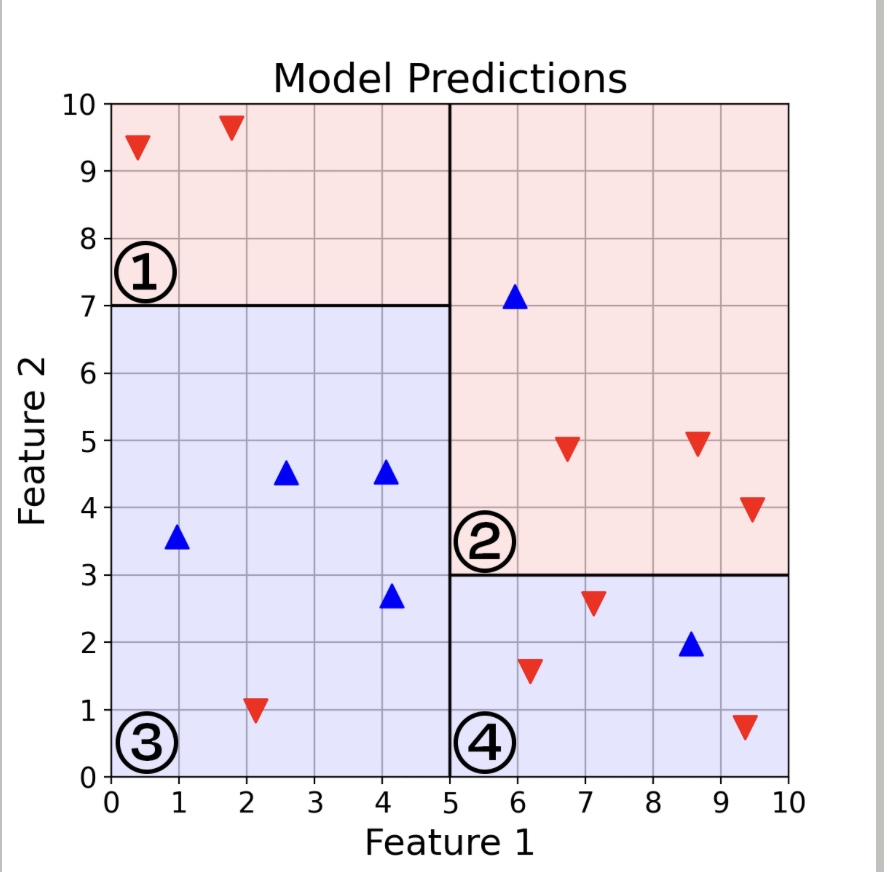
\includegraphics[scale = 0.1]{Images/gini.jpeg}
    \end{center}

\begin{align*}
&\text{Bereich 1: } R = 2, \; B = 0 \\
&p_r = 1.0, \; p_b = 0.0 \\
&G_1 = 1 - \left(\tfrac{\text{Rote Punkte im Bereich}}{\text{Alle Punkte im Bereich}}\right)^2 - \left(\tfrac{\text{Blaue Punkte}}{\text{Alle Punkte im Bereich}}\right)^2 \\
&G_1 = 1 - (1.0^2 + 0.0^2) = 0.00 \\[6pt]
&\text{Bereich 3: } R = 1, \; B = 4 \\
&p_r = \tfrac{1}{5} = 0.2, \; p_b = 0.8 \\
&G_3 = 1 - (0.2^2 + 0.8^2) = 1 - (0.04 + 0.64) = 0.32 \\[6pt]
&\text{Bereich 2: } R = 3, \; B = 1 \\
&p_r = \tfrac{3}{4} = 0.75, \; p_b = 0.25 \\
&G_2 = 1 - (0.75^2 + 0.25^2) = 1 - (0.5625 + 0.0625) = 0.375 \\[6pt]
&\text{Bereich 4: } R = 3, \; B = 1 \\
&p_r = 0.75, \; p_b = 0.25 \\
&G_4 = 1 - (0.75^2 + 0.25^2) = 0.375 \\[12pt]
&\text{Gesamtanzahl: } n_1 = 2, \; n_2 = 4, \; n_3 = 5, \; n_4 = 4, \; N = 15 \\[4pt]
&G_{\text{gesamt}} = \tfrac{n_1}{N} G_1 + \tfrac{n_2}{N} G_2 + \tfrac{n_3}{N} G_3 + \tfrac{n_4}{N} G_4 \\
&\phantom{G_{\text{gesamt}}} = \tfrac{2}{15}(0.00) + \tfrac{4}{15}(0.375) + \tfrac{5}{15}(0.32) + \tfrac{4}{15}(0.375) \\
&\phantom{G_{\text{gesamt}}} = 0 + 0.1000 + 0.1067 + 0.1000 \approx 0.3067 \\[6pt]
&\boxed{G_{\text{gesamt}} \approx 0.31}
\end{align*}
\end{contentbox}

\subsubsection{DP für Linearkombinationen}

\begin{codebox}
    \begin{lstlisting}[style=CodeExpert]
def possible_amounts(max_amount, denominations):
  """example : possible_amounts(20, [5, 2]) returns [0, 2, 4,
  5, 6, 7, 8, 9, 10, 11, 12, 13, 14, 15, 16, 17, 18, 19, 20]
  all linear combinations up to 20 of 5 and 2.
  """
  n = max_amount
  s = [False] * (n + 1)
  s[0] = True

  for i in range(1, n+1):
    s[i] = False
    for d in denominations:
      if i - d >= 0 and s[i - d]:
        s[i] = True
  return s
\end{lstlisting}
\end{codebox}

\subsection{Linked Lists}
\label{sec:12-linked-lists}

\begin{codebox}
\begin{lstlisting}[style=CodeExpert]
    def mergeTwoLists(self, list1: Optional[ListNode], list2:
    Optional[ListNode]) -> Optional[ListNode]:
    # Create a dummy node to start the new list
    dummy = ListNode(0)
    # This will always point to the last node
    last = dummy
    #in the new list
    # Pointer for traversing list1
    p1 = list1
    # Pointer for traversing list2
    p2 = list2

    # Traverse both lists and merge them by comparing node values
    while p1 is not None and p2 is not None:
        if p1.val <= p2.val:
            last.next = p1
            p1 = p1.next
        else:
            last.next = p2
            p2 = p2.next
        last = last.next

    # Attach the remaining nodes of the non-empty list
    if p1 is not None:
        last.next = p1
    else:
        last.next = p2

    return dummy.next
    # The first node is dummy, so return the next node
\end{lstlisting}
\end{codebox}


\subsection{String umkehren}
\label{sec:12-string-umkehren}

\begin{codebox}
\begin{lstlisting}[style=CodeExpert]
#reverses a string cut into intervals: ABCDE
#with interval 2 becomes BADCE
def reverse_string(text, interval):
  reverse = ""
  for i in range(0, len(text), interval):
    reverse += text[i:i+interval:1][::-1]
  return reverse

\end{lstlisting}
\end{codebox}
